In questa sezione verrà studiata la possibilità di inserire un attributo ridondante all'interno del progetto, per sua natura un dato ridondante non dovrebbe servire in quanto calcolabile attraverso una serie di operazioni su dati già presenti, ma a volte il loro numero potrebbe risultare eccessivo. 

Le due operazioni che andremo a studiare sono le funzioni c9 e c10 che chiameremo rispettivamente operazione 1 e 2: 
% \begin{itemize}
%     \item Operazione 1: c9. Lasciare una recensione riguardo un servizio acquistato
%     \item Operazione 2: c10. Visualizzare lista servizi
% \end{itemize}
\begingroup % localize the following settings  
\begin{longtblr}
    [
    caption = {Operazioni richieste dai Clienti},
    label = {tab:Operazioni richieste da cliente},
]{
    colspec = {|X[1]X[8,l]X[3]X[1]X[8,l]|},
    rowhead = 1,
    hlines,
    row{even} = {lightgray},
    row{1} = {MediumSeaGreen},
} 
Cod & Nome Operazione & Freq & Tipo & Descrizione\\
c.9 & Lasciare una recensione riguardo un servizio acquistato & \num{1500} & I & Il cliente rilascia una votazione \\ 
c.10 & Visualizzare lista servizi & \num{7500} & I & Il cliente visualizza la lista dei servizi disponibili \\ 

\end{longtblr}

\endgroup
Da notare che l'operazione 2 dipende dal numero di servizi visualizzati per pagina e dal numero di queste pagine visualizzate durante la ricerca dell'utente. Per i seguenti calcoli verrà presa in considerazione una media di 50 servizi visualizzati per ciascuna operazione 2.  

Si deve decidere se inserire l'attributo votoMedio nell'entità Servizio.\\
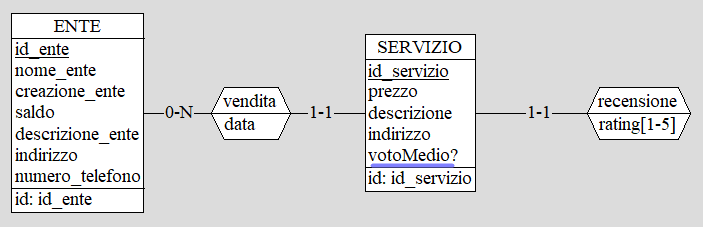
\includegraphics[width=0.95\columnwidth]{ridondanza.png}

\begingroup % localize the following settings  
\setlength{\arrayrulewidth}{0.5mm}
\renewcommand{\arraystretch}{1.5}
\begin{longtblr}
[
caption = {Stima del volume di dati},
label = {tab:Stima del volume di dati},
]{
colspec = {|X[3,l]X[2]X[2]X[6,l]|},
rowhead = 1,
hlines,
row{even} = {PaleTurquoise},
row{1} = {SkyBlue},
} 
Concetto & Costrutto & Volume & Descrizione\\
Ente & Entità & \num{300} & Fornisce i servizi che il cliente usufruisce\\
Servizi & Entità & \num{2400} & Data la cardinalità mi aspetto una stima di 8 servizi ad ente durante l'anno \\
Vendita & Relazione &  \num{1000000} & Si stima che ogni utente attivo compri due servizi ogni giorno in media\\
Recensione & Relazione & \num{500000} & Ogni cliente può lasciare una recensione per servizio acquistato ma non è detto che tutti i clienti lo facciano \\
\end{longtblr}

\endgroup

\subsubsection{Calcolo senza ridondanza}
\begin{longtblr}
[
caption = {Operazione 1 senza ridondanza},
]{
colspec = {|X[3]X[1]X[2]X[4]|},
rowhead = 1,
hlines,
row{even} = {lightgray},
row{1} = {MediumSeaGreen},
} 
Concetto & Costrutto & Accessi & Tipo \\
recensione & R & 1 & S \\
\SetCell[c=4]{l, white} {
    Totale: 1S \textrightarrow 1500/giorno\\
    Costo totale: 1500 x (1 x 2) = 3000/giorno
    }
\end{longtblr}

\begin{longtblr}
[
caption = {Operazione 2 senza ridondanza},
]{
colspec = {|X[3]X[1]X[2]X[4]|},
rowhead = 1,
hlines,
row{even} = {lightgray},
row{1} = {MediumSeaGreen},
} 
Concetto & Costrutto & Accessi & Tipo \\
Servizio & E & \num{50} & L \\
recensione & R & \num{10000} & L \\
\SetCell[c=4]{l, white} {
    Totale: 1S \textrightarrow 7500/giorno\\
    Costo totale: 7500 x (10050) = \num{7875000}/giorno
    }
\end{longtblr}
Il numero totale di accessi giornalieri è \num{7878000}.


\subsubsection{Calcolo con ridondanza}
\begin{longtblr}
    [
    caption = {Operazione 1 con ridondanza},
    ]{
    colspec = {|X[3]X[1]X[2]X[4]|},
    rowhead = 1,
    hlines,
    row{even} = {lightgray},
    row{1} = {MediumSeaGreen},
    } 
    Concetto & Costrutto & Accessi & Tipo \\
    recensione & R & 1 & S \\
    recensione & R & 200 & L \\
    Servizio & R & 1 & S \\
    \SetCell[c=4]{l, white} {
        Totale: 200L + 1S \textrightarrow 1500/giorno\\
        Costo totale: 1500 x (200 + 2 x 2) = \num{306000}/giorno
        }
    \end{longtblr}
    
    \begin{longtblr}
    [
    caption = {Operazione 2 con ridondanza},
    ]{
    colspec = {|X[3]X[1]X[2]X[4]|},
    rowhead = 1,
    hlines,
    row{even} = {lightgray},
    row{1} = {MediumSeaGreen},
    } 
    Concetto & Costrutto & Accessi & Tipo \\
    Servizio & E & \num{50} & L \\
    \SetCell[c=4]{l, white} {
        Totale: 1S \textrightarrow 7500/giorno\\
        Costo totale: 7500 x (50) = \num{375000}/giorno
        }
    \end{longtblr}
Il numero totale di accessi giornalieri è \num{681000}.

\subsubsection{Conclusione}
Dai calcoli fatti è evidente che la soluzione con ridondanza comporta un notevole vantaggio nel numero di accessi giornalieri, riducendo il peso sul database da \num{7878000} a \num{681000}. Alla luce di questo si manterrà la soluzione \ul{con} ridondanza.